\documentclass[UTF-8]{ctexbeamer}
\usetheme{Copenhagen}
\usecolortheme{seahorse}

\usepackage{multimedia}
\usepackage{listings}
\usepackage{minted}
\usepackage{tikz}
\usepackage{textcomp}
\usepackage[normalem]{ulem}

\title{Proof Assistant - A 猫咪 Approach}

\author{喵喵}
\date{2022.3}

\begin{document}

\part{Intro}

\begin{frame}
  \titlepage
  \begin{center}
    
\includegraphics[width=.1\textwidth]{assets/float.png}
  \end{center}
\end{frame}

\begin{frame}
  \frametitle{自我介绍}

  \texttt{喵喵: 猫猫}
\end{frame}

\begin{frame}
  \frametitle{Previously...}

  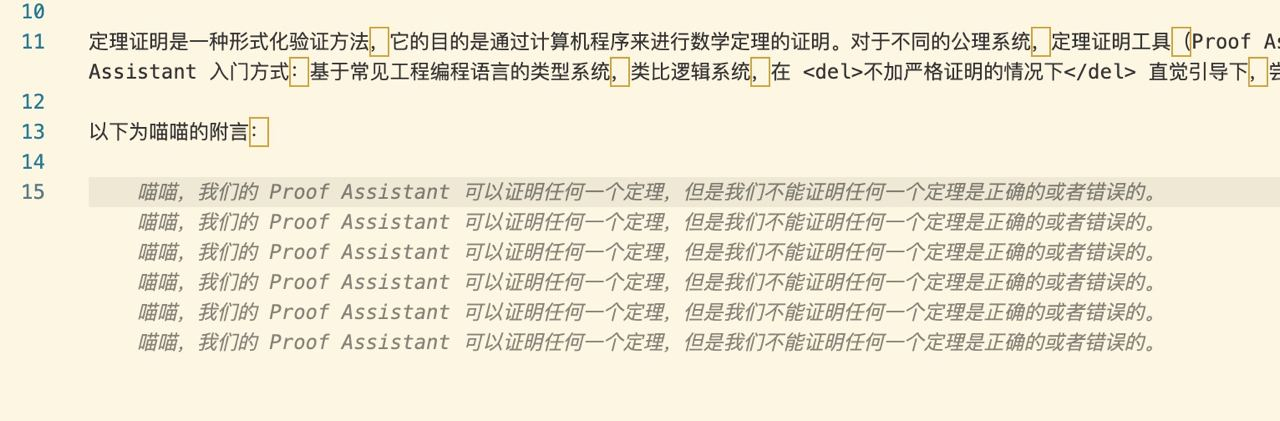
\includegraphics[width=\textwidth]{assets/scary.jpg}

  \pause

  
\includegraphics[width=0.4\textwidth]{assets/gone.png}

  \pause

  \url{https://tuna.moe/event/2020/coq-proof/}
\end{frame}

\begin{frame}
  \frametitle{Motivation}

  \pause
  \begin{figure}
    
\includegraphics[width=0.5\textwidth]{assets/doughnut.png}
    \caption{喵喵 embedded in $S^1 \times D^2$}
  \end{figure}
\end{frame}

\begin{frame}
  \frametitle{Motivation (Cont.)}

  \url{https://github.com/caotic123/PomPom-Language}
  
  \pause

  \vspace{1em}

  能否在 1000 行内使用 Rust 实现一个 Proof Assistant?

  \pause

  \begin{figure}
    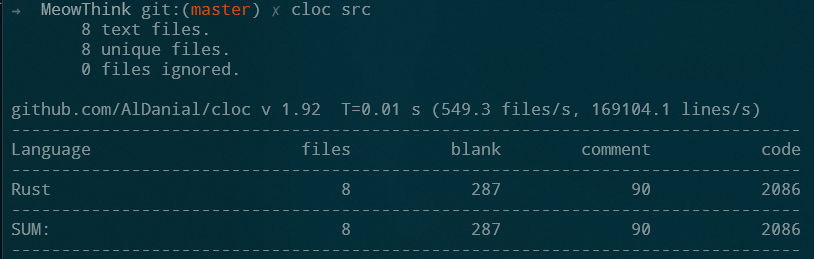
\includegraphics[width=\textwidth]{assets/cloc.png}
    \caption{"2000 LOC can (sort of)"}
  \end{figure}

  \url{https://github.com/CircuitCoder/MeowThink}

\end{frame}

\part{命题逻辑}
\frame{\partpage}

\begin{frame}
  \frametitle{直觉逻辑 - Why}
  
  \pause

  \begin{block}{中国民间数学家定理 (CFMT)}
    任意大于 2 的偶数,都可以表示成两个质数的和。
  \end{block}

  \pause

  \vspace{1em}

  \begin{columns}
    \begin{column}{0.5\textwidth}
      \centering
      "CFMT 和 ZFC 系统独立"

      \pause
      \vspace{0.5em}

      
\includegraphics[width=0.8\textwidth]{assets/le.png}
    \end{column}
    \pause
    \begin{column}{0.5\textwidth}
      \centering
      "CFMT 是哪个公理的结果?"

      \pause
      \vspace{0.5em}

      
\includegraphics[width=0.8\textwidth]{assets/bule.png}
    \end{column}
  \end{columns}
\end{frame}

\begin{frame}
  \frametitle{直觉逻辑 - How}

  经典逻辑:真值表是本质的。

  \begin{center}
  枚举 P, Q 取值可以证明 $ \overline{P \land Q} \rightarrow \overline{P} \lor \overline{Q} $
  \end{center}

  \pause

  直觉逻辑:推理,也就是\textbf{蕴含}($\rightarrow$)是本质的。

  \begin{center}
    如果已知 $P$, 已知 $P \rightarrow Q$, 可以证明 $Q$
  \end{center}

  \pause

  \vspace{1em}

  $$
  \neg A := A \rightarrow \bot
  $$
  $$
  \bot \rightarrow B
  $$

  \pause

  \vspace{1em}

  \begin{center}
    在直觉逻辑中,\textbf{排中律}和\textbf{双重否定去除}不自然成立。
  \end{center}
\end{frame}

\begin{frame}[fragile]
  \frametitle{Curry-Howard 对应}

  \begin{columns}
    \begin{column}{0.5\textwidth}
      $$
      A \rightarrow B
      $$

      \pause

      \textbf{证明方法:} 在已知 A 的情况下,尝试证明 B。

      \pause
      \vspace{0.5em}

      \textbf{使用方法:} 如果拿到了 A 的证明,那么就证出来了 B。
    \end{column}
    \begin{column}{0.5\textwidth}
      \pause
      \centering
      \begin{minted}{rust}
impl Fn(A) -> B
      \end{minted}

      \pause

      \textbf{实现方法:} 在有 A 的情况下,尝试给出类型为 B 的东西。

      \pause
      \vspace{0.5em}

      \textbf{使用方法:} 喂一个 A 类型的东西,吐出一个 B 类型的东西。
    \end{column}
  \end{columns}

  \pause
  \vspace{1em}

  {
    \begin{center}
      \LARGE 直觉逻辑的证明和程序存在一一对应的关系
    \end{center}
  }
\end{frame}

\begin{frame}[fragile]
  \frametitle{We can prove stuff!}

  \begin{minted}{rust}
fn id<A>(a: A) -> A;

fn concat<A, B, C>(
  first: impl Fn(A) -> B,
  second: impl Fn(B) -> C
) -> impl Fn(A) -> C;
  \end{minted}

  \pause

  $$
  A \rightarrow A
  $$
  $$
  (A \rightarrow B) \rightarrow (B \rightarrow C) \rightarrow (A \rightarrow C)
  $$
\end{frame}

\begin{frame}[fragile]
  \frametitle{We can prove stuff!}

  \begin{minted}{rust}
fn id<A>(a: A) -> A;

fn concat<A, B, C>(
  first: A -> B,
  second: B -> C
) -> (A -> C);
  \end{minted}

  $$
  A \rightarrow A
  $$
  $$
  (A \rightarrow B) \rightarrow (B \rightarrow C) \rightarrow (A \rightarrow C)
  $$
\end{frame}

\begin{frame}[fragile]
  \frametitle{$\land, \lor, \top, \bot$}

  \pause
  \begin{minted}{rust}
(A, B)
  \end{minted}

  \pause
  \begin{minted}{rust}
// Case study = match
enum Either<A, B> {
  Left(A),
  Right(B),
}
  \end{minted}

  \pause
  \begin{minted}{rust}
struct Trivial; // Or ()
  \end{minted}

  \pause
  \begin{minted}{rust}
enum False {}; // Or !
  \end{minted}
\end{frame}

\begin{frame}[fragile]
  \frametitle{We can prove (other) stuff}

  \begin{minted}{rust}
fn and_to_or<a, b>(and: (a, b)) -> Either<a, b> {
  Either::left(and.0)
}
  \end{minted}

  $$
  a \land b \rightarrow a \lor b
  $$
\end{frame}

\begin{frame}[fragile]
  \frametitle{We can prove (other) stuff}

  \begin{minted}{rust}
fn and_to_or<A, B>(and: A × B) -> (A + B) {
  Left(and.first)
}
  \end{minted}

  $$
  a \land b \rightarrow a \lor b
  $$
\end{frame}

\begin{frame}[fragile]
  \frametitle{We can prove (other) stuff!}

  \begin{block}{LEM Irrefutable}
  $$
  \neg \neg (P \lor \neg P)
  $$
  \end{block}

  \pause
  \vspace{2em}

  \begin{minted}{rust}
fn lem_irrefutable<P>(
  lem_false: (P + (P -> !)) -> !
) -> ! {
  let p_to_false: P -> !
    = |p: P| lem_false(Left(p));
  lem_false(Right(p_to_false))
}
  \end{minted}
\end{frame}

\begin{frame}[fragile]
  \frametitle{Wait a minute...}

  \pause

  \begin{minted}{rust}
    fn bad<T>(t: T) -> ! {
      loop { /* Meow */ }
    }

    fn worse<T>(t: T) -> ! {
      // Meow meow
      worse(t)
    }
  \end{minted}

  \pause

  \vspace{1em}

  \begin{block}{函数}
    在数学中为两不为空集的集合间的一种对应关系:
    
    输入值集合中的每项元素皆能对应\textbf{唯一一项}输出值集合中的元素。
  \end{block}
\end{frame}

\begin{frame}
  \frametitle{Totality checker}

  递归必须结束。

  \pause

  \vspace{1em}

  检查循环是否终止比较麻烦。
  
  \pause
  
  循环可以用递归替代 - 不允许循环。
\end{frame}

\part{谓词逻辑}
\frame{\partpage}

\begin{frame}
  \frametitle{一阶逻辑?}

  我们如何表示谓词?

  \begin{block}{命题 Even}
    $$
    \text{n 是自然数}, Even(n) \mapsto \text{n 是个偶数}
    $$

    \pause
    \vspace{0.5em}

    $$
    Even: \text{自然数} \rightarrow \text{命题}
    $$

    \pause
    \vspace{0.5em}

    \begin{center}
      \texttt{P: Nat -> Type}
    \end{center}
  \end{block}
\end{frame}

\begin{frame}
  \frametitle{\texttt{Data -> Type}??}

  \pause

  \texttt{Type -> Type}: 泛型 (Generic)

  \pause

  \texttt{Constant -> Type}: Const Generic

  \pause

  \texttt{Data -> Type}: Dependent Typing
\end{frame}

\begin{frame}[fragile]
  \frametitle{Dependent Typing}

  允许:
  \begin{itemize}
    \pause
    \item Dependent Function: \texttt{(a: A) -> P(a)}
    \pause
    \item Dependent Pair: \texttt{(a: A) × P(a)}
  \end{itemize}

  \pause
  \vspace{1em}

  \begin{minted}{rust}
    let dep_fun: (a: A) -> P(a);
    dep_fun(some_a): P(some_a);

    let dep_pair: (a: A) × P(a);
    dep_pair.second: P(dep_pair.first);
  \end{minted}

  \pause
  \vspace{1em}

  量词:$\forall, \exists$

\end{frame}

\begin{frame}[fragile]
  \frametitle{类型表示}

  \begin{minted}{rust}
fn id<A>(a: A) -> A;
  \end{minted}

  \pause
  $\Downarrow$

  \texttt{id<A>: A -> A}

  \pause

  $\Downarrow$

  \texttt{id: (A: Type) -> A -> A}

  \pause
  $\Downarrow$

  \begin{minted}{rust}
fn id(A: Type, a: A) -> A;
  \end{minted}
\end{frame}

\begin{frame}[fragile]
  \frametitle{We can prove (more) stuff!}

  \begin{block}{Axiom of Choice...?}
  如果对于一组集合 S(i) 中的每一个,都可以选出来一个元素 s 满足 P(i, s),那么存在一个选择函数,从每个 S(i) 中选出一个,使得每个选择的结果都满足谓词 P
  \end{block}

  \pause

  $$
  \begin{aligned}
  &\forall i \in I, \exists s \in S(i), P(i, s) \\
  &\rightarrow \\
  &\exists f: ((i: I) \rightarrow S(i)) \\
  &\forall i \in I, P(i, f(i))
  \end{aligned}
  $$
\end{frame}

\begin{frame}[fragile]
  \frametitle{We can prove (more) stuff!}

  \begin{minted}{rust}
fn not_exactly_choice(
  Index: Type,
  Set: Index -> Type,
  Pred: Index -> Set -> Type,

  all_has_elem: (
    (i: Index)
    -> ((s: Set(i)) × Pred(i, s))
  )
) -> (
  (f: (i: Index) -> Set(i))
  × ((any: Index) -> Pred(any, f(any)))
);
  \end{minted}
\end{frame}

\begin{frame}
  \frametitle{相等}

  \pause
  \begin{figure}
    
\includegraphics[width=0.5\textwidth]{assets/same.png}
    \caption{\texttt{m ==(T) n}}
  \end{figure}
\end{frame}

\begin{frame}
  \frametitle{相等}

  $$
  \forall n: Nat, \forall m: Nat, (n \equiv m) \rightarrow (2n \equiv 2m)
  $$

  \pause

  \texttt{(n: Nat) -> (m: Nat)}

  \texttt{    -> (n ==(Nat) m)}

  \texttt{    -> (double(n) ==(Nat) double(m))}
\end{frame}

\begin{frame}
  \frametitle{相等的行为}

  \begin{center}
    \texttt{==(\_): (T: Type) -> (lhs: T) -> (rhs: T) -> Type}
  \end{center}

  \pause
  \begin{itemize}
    \item 自反性
    
    \texttt{refl: (T: Type) -> (x: T) -> (x ==(T) x)}

    \pause
    \item 类型转换
    
    \texttt{cast: (T: Type) -> (U: Type) -> (T ==(Type) U) -> T -> U}

    \pause
    \item 映射后不变
    
    \texttt{ap: (f: T -> U) -> (a ==(T) b) -> (f(a) ==(U) f(b))}
  \end{itemize}
\end{frame}

\begin{frame}[fragile]
  \frametitle{对称性 / 传递性在哪里?}

  \pause

  \begin{minted}{rust}
fn eq_sym(
  T: Type,
  a: T, b: T,
  eq: a ==(T) b,
) -> b ==(T) a {
  \end{minted}
  \pause
  \begin{minted}{rust}
  let start: (a ==(T) a) = refl(T, a);
  \end{minted}
  \pause
  \begin{minted}{rust}
  let ty_eq: (a ==(T) a) ==(Type) (b ==(T) a)
    = ap(|x: T| { x ==(T) a}, eq);
  \end{minted}
  \pause
  \begin{minted}{rust}
  cast(/* ... */, ty_eq, start)
}
  \end{minted}
\end{frame}

\begin{frame}[fragile]
  \frametitle{We can prove (even more) stuff}

  \begin{minted}{rust}
enum C3 {
  Zero, One, Two,
}
// Define mul: C3 -> C3 -> C3

fn C3_order_3(
  input: C3
) -> mul(mul(input, input), input) ==(C3) C3::Zero;
  \end{minted}
  

\end{frame}

\part{归纳}
\frame{\partpage}

\begin{frame}[fragile]
  \frametitle{归纳定义 / 证明}

  \pause

  回忆自然数的定义:
  \begin{itemize}
    \item 0 是自然数。
    \item 如果 $n$ 是自然数,那么 $n$ 的后继是自然数。
  \end{itemize}

  \pause

  \begin{minted}{rust}
enum Nat {
  Zero,
  Succ(Nat),
}
  \end{minted}
\end{frame}

\begin{frame}[fragile]
  \frametitle{使用 Nat 的函数}

  \begin{minted}{rust}
fn add(a: Nat, b: Nat) -> Nat {
  match a {
    Nat::Zero => b,
    Nat::Succ(prev) => Nat::Succ(add(prev, b)),
  }
}
  \end{minted}

  \pause

  递归 = 归纳定义
\end{frame}

\begin{frame}[fragile]
  \frametitle{使用 Nat 的函数}
  \begin{minted}{rust}
fn add_zero(a: Nat)
  -> (add(a, Nat::Zero) == a) {
    match a {
      Nat::Zero => refl(Nat, Nat::Zero),
      Nat::Succ(prev) => ap(Nat::Succ, add_zero(prev)),
    }
  }
  \end{minted}
  \pause

  递归 = 归纳证明
\end{frame}

\part{公理}
\frame{\partpage}

\begin{frame}
  \frametitle{公理}

  "存在一个类型是 ... 的项"

  \pause

  不一定会导致不可计算性。
\end{frame}

\begin{frame}
  \frametitle{排中律}

  \begin{itemize}
    \item \texttt{lem: (P + !P)}
    \item \texttt{dne: !!P -> P}
    \item \texttt{peirce: ((P -> Q) -> P) -> P}
    \item \texttt{implies: (P -> Q) -> (Q + !P)}
    \item \texttt{de\_morgan: !(!P × !Q) -> P + Q}
  \end{itemize}
\end{frame}

\begin{frame}
  \frametitle{外延性}

  $\{2x | x \in \mathbb{Z}\} =? \{2x + 2 | x \in \mathbb{Z}\}$
  \pause

  简单算法 =? 快速幂

  \pause

  \begin{itemize}
    \item 命题外延性: \texttt{(P -> Q) × (Q -> P) -> P = Q}
    \pause
    \item 函数外延性: \texttt{(a -> f(a) == g(a)) -> f == g}
    \pause
    \item Univalence(类型外延性): $(A \simeq B) \simeq (A = B)$
  \end{itemize}
\end{frame}

\part{碎碎念}
\frame{\partpage}

\begin{frame}
  \frametitle{What is \texttt{Type}}

  \pause
  \begin{itemize}
    \item \texttt{Type: Type}

    \pause
    "The set of all sets"

    \pause
    非直谓性(Impredicativity) \& \texttt{Girard's paradox}

    \item \texttt{Type} 是特殊的

    "The \textbf{class} of all sets"

    \pause
    "\texttt{List<Type>}"

    \pause
    \item \texttt{Type 0} $\in$ \texttt{Type 1} $\in$ \texttt{Type 2} ...



  \end{itemize}
\end{frame}

\begin{frame}
  \frametitle{Axiom K \& HoTT}
  \texttt{\_ ==(a ==(T) b) \_}

  \pause

  \begin{figure}
    
\includegraphics[width=0.5\textwidth]{assets/real.jpg}
    \caption{HoTT}
  \end{figure}
  类型 = 拓扑空间,相等 = 路径,\texttt{ap} = 函数都是连续的。
\end{frame}

\begin{frame}
  \frametitle{That's All!}
  \begin{center}
    
\includegraphics[width=.5\textwidth]{assets/look.png}

    Question time!
  \end{center}
  \url{https://github.com/CircuitCoder/MeowThink}
  \url{https://github.com/CircuitCoder/LocalNeko}
\end{frame}

\end{document}